% AUTO-GENERATED by code/figlib.py helpers -- do not edit
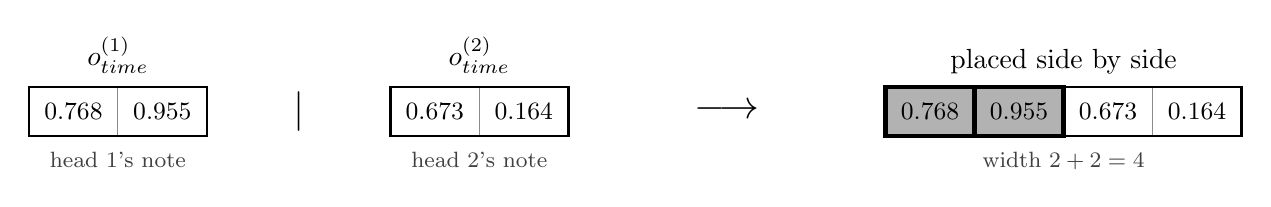
\begin{tikzpicture}
\draw[black!45, fill=white] (0.000,0.310) rectangle (1.130,-0.310);
\node[font=\small, text=black] at (0.565,0.000) {$0.768$};
\draw[black!45, fill=white] (1.130,0.310) rectangle (2.260,-0.310);
\node[font=\small, text=black] at (1.695,0.000) {$0.955$};
\draw[line width=0.9pt] (0.000,0.310) rectangle (2.260,-0.310);
\node[anchor=south, font=\normalsize] at (1.130,0.360) {$\bm o^{(1)}_{\text{time}}$};
\node[anchor=north, font=\footnotesize, text=black!75] at (1.130,-0.390) {head 1's note};
\node[font=\Large] at (3.425,0) {$\big|$};
\draw[black!45, fill=white] (4.590,0.310) rectangle (5.720,-0.310);
\node[font=\small, text=black] at (5.155,0.000) {$0.673$};
\draw[black!45, fill=white] (5.720,0.310) rectangle (6.850,-0.310);
\node[font=\small, text=black] at (6.285,0.000) {$0.164$};
\draw[line width=0.9pt] (4.590,0.310) rectangle (6.850,-0.310);
\node[anchor=south, font=\normalsize] at (5.720,0.360) {$\bm o^{(2)}_{\text{time}}$};
\node[anchor=north, font=\footnotesize, text=black!75] at (5.720,-0.390) {head 2's note};
\node[font=\Large] at (8.865,0) {$\longrightarrow$};
\draw[black!45, fill=black!30] (10.880,0.310) rectangle (12.010,-0.310);
\node[font=\small, text=black] at (11.445,0.000) {$0.768$};
\draw[black!45, fill=black!30] (12.010,0.310) rectangle (13.140,-0.310);
\node[font=\small, text=black] at (12.575,0.000) {$0.955$};
\draw[black!45, fill=white] (13.140,0.310) rectangle (14.270,-0.310);
\node[font=\small, text=black] at (13.705,0.000) {$0.673$};
\draw[black!45, fill=white] (14.270,0.310) rectangle (15.400,-0.310);
\node[font=\small, text=black] at (14.835,0.000) {$0.164$};
\draw[line width=1.6pt] (10.880,0.310) rectangle (12.010,-0.310);
\draw[line width=1.6pt] (12.010,0.310) rectangle (13.140,-0.310);
\draw[line width=0.9pt] (10.880,0.310) rectangle (15.400,-0.310);
\node[anchor=south, font=\normalsize] at (13.140,0.360) {placed side by side};
\node[anchor=north, font=\footnotesize, text=black!75] at (13.140,-0.390) {width $2+2=4$};
\end{tikzpicture}
\\[10pt]
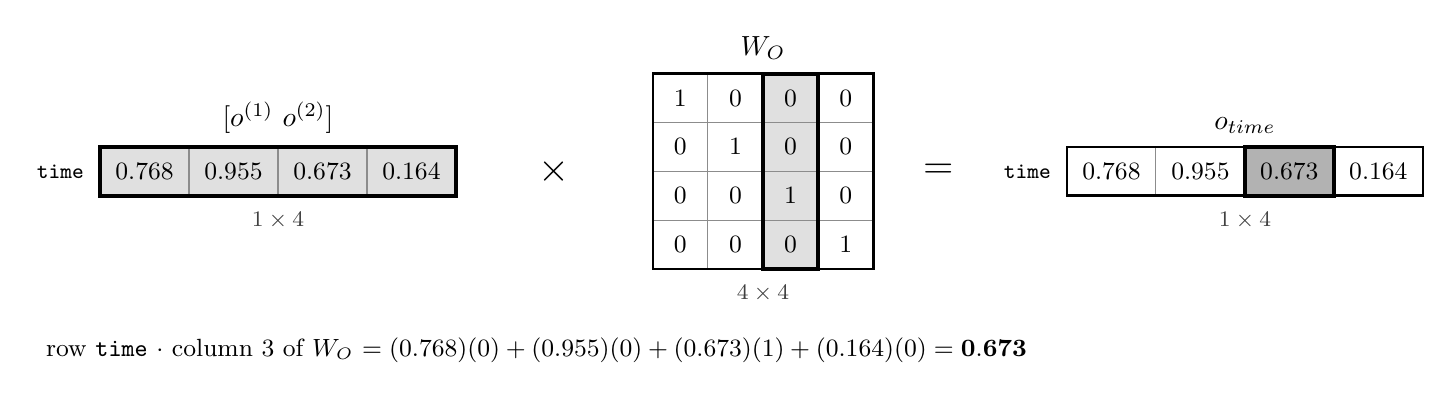
\begin{tikzpicture}
\draw[black!45, fill=black!12] (0.810,0.310) rectangle (1.940,-0.310);
\node[font=\small, text=black] at (1.375,0.000) {$0.768$};
\draw[black!45, fill=black!12] (1.940,0.310) rectangle (3.070,-0.310);
\node[font=\small, text=black] at (2.505,0.000) {$0.955$};
\draw[black!45, fill=black!12] (3.070,0.310) rectangle (4.200,-0.310);
\node[font=\small, text=black] at (3.635,0.000) {$0.673$};
\draw[black!45, fill=black!12] (4.200,0.310) rectangle (5.330,-0.310);
\node[font=\small, text=black] at (4.765,0.000) {$0.164$};
\draw[line width=1.4pt] (0.810,0.310) rectangle (5.330,-0.310);
\draw[line width=0.9pt] (0.810,0.310) rectangle (5.330,-0.310);
\node[anchor=east, font=\footnotesize\ttfamily] at (0.730,0.000) {time};
\node[anchor=south, font=\normalsize] at (3.070,0.360) {$[\bm o^{(1)}\ \bm o^{(2)}]$};
\node[anchor=north, font=\footnotesize, text=black!75] at (3.070,-0.390) {$1\times4$};
\node[font=\Large] at (6.580,0) {$\times$};
\draw[black!45, fill=white] (7.830,1.240) rectangle (8.530,0.620);
\node[font=\small, text=black] at (8.180,0.930) {$1$};
\draw[black!45, fill=white] (8.530,1.240) rectangle (9.230,0.620);
\node[font=\small, text=black] at (8.880,0.930) {$0$};
\draw[black!45, fill=black!12] (9.230,1.240) rectangle (9.930,0.620);
\node[font=\small, text=black] at (9.580,0.930) {$0$};
\draw[black!45, fill=white] (9.930,1.240) rectangle (10.630,0.620);
\node[font=\small, text=black] at (10.280,0.930) {$0$};
\draw[black!45, fill=white] (7.830,0.620) rectangle (8.530,0.000);
\node[font=\small, text=black] at (8.180,0.310) {$0$};
\draw[black!45, fill=white] (8.530,0.620) rectangle (9.230,0.000);
\node[font=\small, text=black] at (8.880,0.310) {$1$};
\draw[black!45, fill=black!12] (9.230,0.620) rectangle (9.930,0.000);
\node[font=\small, text=black] at (9.580,0.310) {$0$};
\draw[black!45, fill=white] (9.930,0.620) rectangle (10.630,0.000);
\node[font=\small, text=black] at (10.280,0.310) {$0$};
\draw[black!45, fill=white] (7.830,0.000) rectangle (8.530,-0.620);
\node[font=\small, text=black] at (8.180,-0.310) {$0$};
\draw[black!45, fill=white] (8.530,0.000) rectangle (9.230,-0.620);
\node[font=\small, text=black] at (8.880,-0.310) {$0$};
\draw[black!45, fill=black!12] (9.230,0.000) rectangle (9.930,-0.620);
\node[font=\small, text=black] at (9.580,-0.310) {$1$};
\draw[black!45, fill=white] (9.930,0.000) rectangle (10.630,-0.620);
\node[font=\small, text=black] at (10.280,-0.310) {$0$};
\draw[black!45, fill=white] (7.830,-0.620) rectangle (8.530,-1.240);
\node[font=\small, text=black] at (8.180,-0.930) {$0$};
\draw[black!45, fill=white] (8.530,-0.620) rectangle (9.230,-1.240);
\node[font=\small, text=black] at (8.880,-0.930) {$0$};
\draw[black!45, fill=black!12] (9.230,-0.620) rectangle (9.930,-1.240);
\node[font=\small, text=black] at (9.580,-0.930) {$0$};
\draw[black!45, fill=white] (9.930,-0.620) rectangle (10.630,-1.240);
\node[font=\small, text=black] at (10.280,-0.930) {$1$};
\draw[line width=1.4pt] (9.230,1.240) rectangle (9.930,-1.240);
\draw[line width=0.9pt] (7.830,1.240) rectangle (10.630,-1.240);
\node[anchor=south, font=\normalsize] at (9.230,1.290) {$W_O$};
\node[anchor=north, font=\footnotesize, text=black!75] at (9.230,-1.320) {$4\times4$};
\node[font=\Large] at (11.455,0) {$=$};
\draw[black!45, fill=white] (13.090,0.310) rectangle (14.220,-0.310);
\node[font=\small, text=black] at (13.655,0.000) {$0.768$};
\draw[black!45, fill=white] (14.220,0.310) rectangle (15.350,-0.310);
\node[font=\small, text=black] at (14.785,0.000) {$0.955$};
\draw[black!45, fill=black!30] (15.350,0.310) rectangle (16.480,-0.310);
\node[font=\small, text=black] at (15.915,0.000) {$0.673$};
\draw[black!45, fill=white] (16.480,0.310) rectangle (17.610,-0.310);
\node[font=\small, text=black] at (17.045,0.000) {$0.164$};
\draw[line width=1.6pt] (15.350,0.310) rectangle (16.480,-0.310);
\draw[line width=0.9pt] (13.090,0.310) rectangle (17.610,-0.310);
\node[anchor=east, font=\footnotesize\ttfamily] at (13.010,0.000) {time};
\node[anchor=south, font=\normalsize] at (15.350,0.360) {$\bm o_{\text{time}}$};
\node[anchor=north, font=\footnotesize, text=black!75] at (15.350,-0.390) {$1\times4$};
\node[anchor=north west, font=\small, align=left] at (0,-1.990) {row \texttt{time} $\cdot$ column 3 of $W_O$ $= (0.768)(0) + (0.955)(0) + (0.673)(1) + (0.164)(0) = \mathbf{0.673}$};
\end{tikzpicture}
